\documentclass[twoside]{book}

% Packages required by doxygen
\usepackage{fixltx2e}
\usepackage{calc}
\usepackage{doxygen}
\usepackage[export]{adjustbox} % also loads graphicx
\usepackage{graphicx}
\usepackage[utf8]{inputenc}
\usepackage{makeidx}
\usepackage{multicol}
\usepackage{multirow}
\PassOptionsToPackage{warn}{textcomp}
\usepackage{textcomp}
\usepackage[nointegrals]{wasysym}
\usepackage[table]{xcolor}

% NLS support packages
\usepackage{polski}
\usepackage[T1]{fontenc}

% Font selection
\usepackage[T1]{fontenc}
\usepackage[scaled=.90]{helvet}
\usepackage{courier}
\usepackage{amssymb}
\usepackage{sectsty}
\renewcommand{\familydefault}{\sfdefault}
\allsectionsfont{%
  \fontseries{bc}\selectfont%
  \color{darkgray}%
}
\renewcommand{\DoxyLabelFont}{%
  \fontseries{bc}\selectfont%
  \color{darkgray}%
}
\newcommand{\+}{\discretionary{\mbox{\scriptsize$\hookleftarrow$}}{}{}}

% Page & text layout
\usepackage{geometry}
\geometry{%
  a4paper,%
  top=2.5cm,%
  bottom=2.5cm,%
  left=2.5cm,%
  right=2.5cm%
}
\tolerance=750
\hfuzz=15pt
\hbadness=750
\setlength{\emergencystretch}{15pt}
\setlength{\parindent}{0cm}
\setlength{\parskip}{3ex plus 2ex minus 2ex}
\makeatletter
\renewcommand{\paragraph}{%
  \@startsection{paragraph}{4}{0ex}{-1.0ex}{1.0ex}{%
    \normalfont\normalsize\bfseries\SS@parafont%
  }%
}
\renewcommand{\subparagraph}{%
  \@startsection{subparagraph}{5}{0ex}{-1.0ex}{1.0ex}{%
    \normalfont\normalsize\bfseries\SS@subparafont%
  }%
}
\makeatother

% Headers & footers
\usepackage{fancyhdr}
\pagestyle{fancyplain}
\fancyhead[LE]{\fancyplain{}{\bfseries\thepage}}
\fancyhead[CE]{\fancyplain{}{}}
\fancyhead[RE]{\fancyplain{}{\bfseries\leftmark}}
\fancyhead[LO]{\fancyplain{}{\bfseries\rightmark}}
\fancyhead[CO]{\fancyplain{}{}}
\fancyhead[RO]{\fancyplain{}{\bfseries\thepage}}
\fancyfoot[LE]{\fancyplain{}{}}
\fancyfoot[CE]{\fancyplain{}{}}
\fancyfoot[RE]{\fancyplain{}{\bfseries\scriptsize Wygenerowano przez Doxygen }}
\fancyfoot[LO]{\fancyplain{}{\bfseries\scriptsize Wygenerowano przez Doxygen }}
\fancyfoot[CO]{\fancyplain{}{}}
\fancyfoot[RO]{\fancyplain{}{}}
\renewcommand{\footrulewidth}{0.4pt}
\renewcommand{\chaptermark}[1]{%
  \markboth{#1}{}%
}
\renewcommand{\sectionmark}[1]{%
  \markright{\thesection\ #1}%
}

% Indices & bibliography
\usepackage{natbib}
\usepackage[titles]{tocloft}
\setcounter{tocdepth}{3}
\setcounter{secnumdepth}{5}
\makeindex

% Hyperlinks (required, but should be loaded last)
\usepackage{ifpdf}
\ifpdf
  \usepackage[pdftex,pagebackref=true]{hyperref}
\else
  \usepackage[ps2pdf,pagebackref=true]{hyperref}
\fi
\hypersetup{%
  colorlinks=true,%
  linkcolor=blue,%
  citecolor=blue,%
  unicode%
}

% Custom commands
\newcommand{\clearemptydoublepage}{%
  \newpage{\pagestyle{empty}\cleardoublepage}%
}

\usepackage{caption}
\captionsetup{labelsep=space,justification=centering,font={bf},singlelinecheck=off,skip=4pt,position=top}

%===== C O N T E N T S =====

\begin{document}

% Titlepage & ToC
\hypersetup{pageanchor=false,
             bookmarksnumbered=true,
             pdfencoding=unicode
            }
\pagenumbering{roman}
\begin{titlepage}
\vspace*{7cm}
\begin{center}%
{\Large Porównywarka postaci do League of Legends }\\
\vspace*{1cm}
{\large Wygenerowano przez Doxygen 1.8.11}\\
\end{center}
\end{titlepage}
\clearemptydoublepage
\tableofcontents
\clearemptydoublepage
\pagenumbering{arabic}
\hypersetup{pageanchor=true}

%--- Begin generated contents ---
\chapter{Dokumentacja programu \char`\"{}\+Porownywarka do League of Legends\char`\"{}}
\label{index}\hypertarget{index}{}Projekt koncowy -\/ Inzynieria Oprogramowania

\begin{DoxyAuthor}{Autor}
Lukasz Kokosza 

Cezary Chmielarz 

Jakub Firlej
\end{DoxyAuthor}
Inzynieria Obliczeniowa 
\chapter{Indeks hierarchiczny}
\section{Hierarchia klas}
Ta lista dziedziczenia posortowana jest z grubsza, choć nie całkowicie, alfabetycznie\+:\begin{DoxyCompactList}
\item \contentsline{section}{Ekwipunek}{\pageref{class_ekwipunek}}{}
\begin{DoxyCompactList}
\item \contentsline{section}{Postac\+\_\+uzytkownika}{\pageref{class_postac__uzytkownika}}{}
\item \contentsline{section}{Przeciwnik}{\pageref{class_przeciwnik}}{}
\end{DoxyCompactList}
\item \contentsline{section}{Generator}{\pageref{class_generator}}{}
\item \contentsline{section}{Porownywarka}{\pageref{class_porownywarka}}{}
\item \contentsline{section}{postac}{\pageref{classpostac}}{}
\begin{DoxyCompactList}
\item \contentsline{section}{Postac\+\_\+uzytkownika}{\pageref{class_postac__uzytkownika}}{}
\item \contentsline{section}{Przeciwnik}{\pageref{class_przeciwnik}}{}
\end{DoxyCompactList}
\item \contentsline{section}{Statystyki}{\pageref{class_statystyki}}{}
\begin{DoxyCompactList}
\item \contentsline{section}{Postac\+\_\+uzytkownika}{\pageref{class_postac__uzytkownika}}{}
\item \contentsline{section}{Przeciwnik}{\pageref{class_przeciwnik}}{}
\end{DoxyCompactList}
\item \contentsline{section}{wyswietlanie}{\pageref{classwyswietlanie}}{}
\begin{DoxyCompactList}
\item \contentsline{section}{Postac\+\_\+uzytkownika}{\pageref{class_postac__uzytkownika}}{}
\item \contentsline{section}{Przeciwnik}{\pageref{class_przeciwnik}}{}
\end{DoxyCompactList}
\end{DoxyCompactList}

\chapter{Indeks klas}
\section{Lista klas}
Tutaj znajdują się klasy, struktury, unie i interfejsy wraz z ich krótkimi opisami\+:\begin{DoxyCompactList}
\item\contentsline{section}{\hyperlink{class_ekwipunek}{Ekwipunek} }{\pageref{class_ekwipunek}}{}
\item\contentsline{section}{\hyperlink{class_generator}{Generator} }{\pageref{class_generator}}{}
\item\contentsline{section}{\hyperlink{class_porownywarka}{Porownywarka} }{\pageref{class_porownywarka}}{}
\item\contentsline{section}{\hyperlink{classpostac}{postac} }{\pageref{classpostac}}{}
\item\contentsline{section}{\hyperlink{class_postac__uzytkownika}{Postac\+\_\+uzytkownika} }{\pageref{class_postac__uzytkownika}}{}
\item\contentsline{section}{\hyperlink{class_przeciwnik}{Przeciwnik} }{\pageref{class_przeciwnik}}{}
\item\contentsline{section}{\hyperlink{class_statystyki}{Statystyki} }{\pageref{class_statystyki}}{}
\item\contentsline{section}{\hyperlink{classwyswietlanie}{wyswietlanie} }{\pageref{classwyswietlanie}}{}
\end{DoxyCompactList}

\chapter{Dokumentacja klas}
\hypertarget{class_ekwipunek}{}\section{Dokumentacja klasy Ekwipunek}
\label{class_ekwipunek}\index{Ekwipunek@{Ekwipunek}}
Diagram dziedziczenia dla Ekwipunek\begin{figure}[H]
\begin{center}
\leavevmode
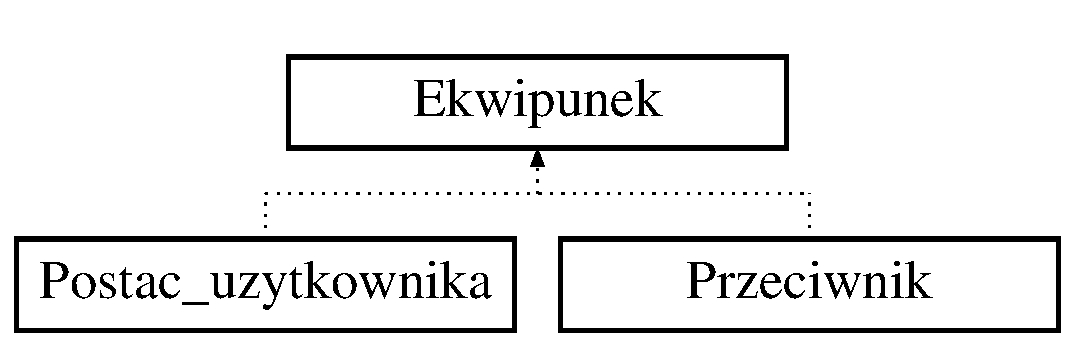
\includegraphics[height=2.000000cm]{class_ekwipunek}
\end{center}
\end{figure}
\subsection*{Atrybuty publiczne}
\begin{DoxyCompactItemize}
\item 
double {\bfseries miecz}\hypertarget{class_ekwipunek_aca4975f90530d108ae70fb56145c1763}{}\label{class_ekwipunek_aca4975f90530d108ae70fb56145c1763}

\item 
string {\bfseries nazwa\+Miecza}\hypertarget{class_ekwipunek_a3d8fdbdf8c9b1a28187840a8ad5e1493}{}\label{class_ekwipunek_a3d8fdbdf8c9b1a28187840a8ad5e1493}

\item 
double {\bfseries luk}\hypertarget{class_ekwipunek_abaf53911fe252142e6de98036e0499c9}{}\label{class_ekwipunek_abaf53911fe252142e6de98036e0499c9}

\item 
string {\bfseries nazwa\+Luku}\hypertarget{class_ekwipunek_a8f9339fade90a85b6ff678a0cb93c61a}{}\label{class_ekwipunek_a8f9339fade90a85b6ff678a0cb93c61a}

\item 
double {\bfseries zbroja}\hypertarget{class_ekwipunek_a4b3354debef86467e856ea0a06cc980f}{}\label{class_ekwipunek_a4b3354debef86467e856ea0a06cc980f}

\item 
string {\bfseries nazwa\+Zbroi}\hypertarget{class_ekwipunek_a455a15b265037ca6140a7e2d3b7d4101}{}\label{class_ekwipunek_a455a15b265037ca6140a7e2d3b7d4101}

\item 
double {\bfseries buty}\hypertarget{class_ekwipunek_a1f627e7d9f730776c37cce40522c82eb}{}\label{class_ekwipunek_a1f627e7d9f730776c37cce40522c82eb}

\item 
string {\bfseries nazwa\+Butow}\hypertarget{class_ekwipunek_a2aafba446378a5eddda44f538c1cf4e5}{}\label{class_ekwipunek_a2aafba446378a5eddda44f538c1cf4e5}

\end{DoxyCompactItemize}


Dokumentacja dla tej klasy została wygenerowana z pliku\+:\begin{DoxyCompactItemize}
\item 
Ekwipunek.\+h\end{DoxyCompactItemize}

\hypertarget{class_generator}{}\section{Dokumentacja klasy Generator}
\label{class_generator}\index{Generator@{Generator}}
\subsection*{Metody publiczne}
\begin{DoxyCompactItemize}
\item 
void {\bfseries Generuj\+Postacie} (\hyperlink{class_postac__uzytkownika}{Postac\+\_\+uzytkownika} \&p1, \hyperlink{class_przeciwnik}{Przeciwnik} \&p2)\hypertarget{class_generator_ad19b0b8c4736de13184492b1f8c7774e}{}\label{class_generator_ad19b0b8c4736de13184492b1f8c7774e}

\end{DoxyCompactItemize}


Dokumentacja dla tej klasy została wygenerowana z plików\+:\begin{DoxyCompactItemize}
\item 
Generator.\+h\item 
Generator.\+cpp\end{DoxyCompactItemize}

\hypertarget{class_porownywarka}{}\section{Dokumentacja klasy Porownywarka}
\label{class_porownywarka}\index{Porownywarka@{Porownywarka}}
\subsection*{Metody publiczne}
\begin{DoxyCompactItemize}
\item 
void {\bfseries Porownaj} (\hyperlink{class_postac__uzytkownika}{Postac\+\_\+uzytkownika} \&p1, \hyperlink{class_przeciwnik}{Przeciwnik} \&p2)\hypertarget{class_porownywarka_aeb3991fd4e8c5b7f3ab1100dd9a0aac0}{}\label{class_porownywarka_aeb3991fd4e8c5b7f3ab1100dd9a0aac0}

\end{DoxyCompactItemize}


Dokumentacja dla tej klasy została wygenerowana z plików\+:\begin{DoxyCompactItemize}
\item 
Porownywarka.\+h\item 
Porownywarka.\+cpp\end{DoxyCompactItemize}

\hypertarget{classpostac}{}\section{Dokumentacja klasy postac}
\label{classpostac}\index{postac@{postac}}
Diagram dziedziczenia dla postac\begin{figure}[H]
\begin{center}
\leavevmode
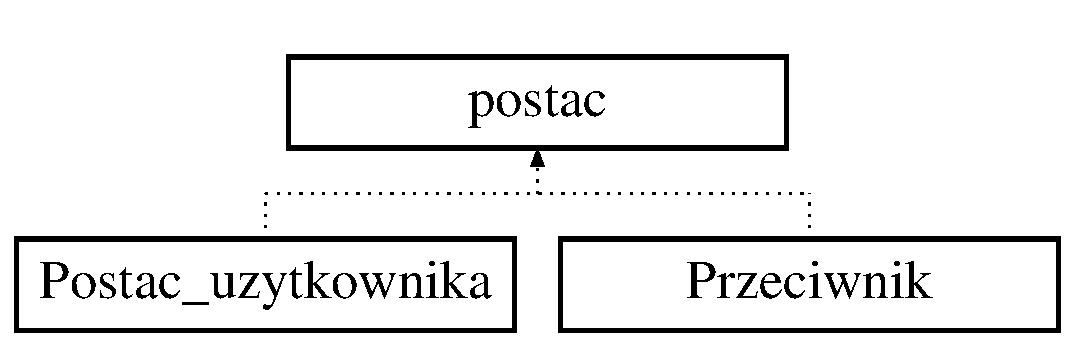
\includegraphics[height=2.000000cm]{classpostac}
\end{center}
\end{figure}
\subsection*{Metody publiczne}
\begin{DoxyCompactItemize}
\item 
virtual void {\bfseries wybierz\+Postac} ()=0\hypertarget{classpostac_a9c9d54380373bf15e9fdb18a1ef8ff91}{}\label{classpostac_a9c9d54380373bf15e9fdb18a1ef8ff91}

\item 
virtual void {\bfseries poczatkowe\+Staty} (int w, int p)=0\hypertarget{classpostac_a7f206bd087f4cb57d716c5ff663746f2}{}\label{classpostac_a7f206bd087f4cb57d716c5ff663746f2}

\item 
virtual void {\bfseries ekwipunek\+Postaci} (string \hyperlink{classpostac}{postac})=0\hypertarget{classpostac_a0020fb6dcc24a9ee0a6ceee7dc91b5cb}{}\label{classpostac_a0020fb6dcc24a9ee0a6ceee7dc91b5cb}

\end{DoxyCompactItemize}


Dokumentacja dla tej klasy została wygenerowana z pliku\+:\begin{DoxyCompactItemize}
\item 
Postac.\+h\end{DoxyCompactItemize}

\hypertarget{class_postac__uzytkownika}{}\section{Dokumentacja klasy Postac\+\_\+uzytkownika}
\label{class_postac__uzytkownika}\index{Postac\+\_\+uzytkownika@{Postac\+\_\+uzytkownika}}
Diagram dziedziczenia dla Postac\+\_\+uzytkownika\begin{figure}[H]
\begin{center}
\leavevmode
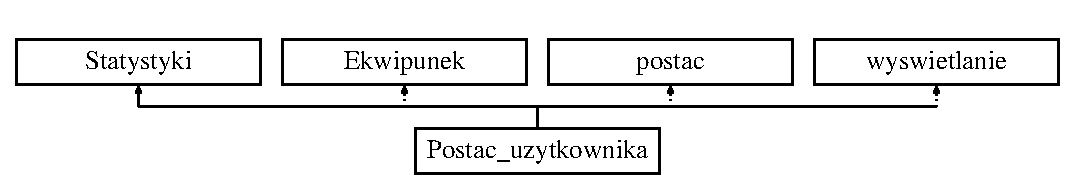
\includegraphics[height=2.000000cm]{class_postac__uzytkownika}
\end{center}
\end{figure}
\subsection*{Metody publiczne}
\begin{DoxyCompactItemize}
\item 
{\bfseries Postac\+\_\+uzytkownika} (string nazwa=\char`\"{}Uzytkownik\char`\"{}, int poziom=5)\hypertarget{class_postac__uzytkownika_a82711323bfb499ed192674bc552d503f}{}\label{class_postac__uzytkownika_a82711323bfb499ed192674bc552d503f}

\item 
void {\bfseries wybierz\+Postac} ()\hypertarget{class_postac__uzytkownika_a2f62bd3ed60202156657217a710b4bb2}{}\label{class_postac__uzytkownika_a2f62bd3ed60202156657217a710b4bb2}

\item 
double {\bfseries algorytm\+Obliczenia\+Procentu} (int p)\hypertarget{class_postac__uzytkownika_ae36ae0e7edd1bb7392bb79095e8d06a9}{}\label{class_postac__uzytkownika_ae36ae0e7edd1bb7392bb79095e8d06a9}

\item 
double {\bfseries opoznienie\+Ataku} (double predkosc, int poziom, double procent)\hypertarget{class_postac__uzytkownika_af0e35bb1670f52785a2de82945a9832a}{}\label{class_postac__uzytkownika_af0e35bb1670f52785a2de82945a9832a}

\item 
void {\bfseries poczatkowe\+Staty} (int w, int p)\hypertarget{class_postac__uzytkownika_aec17a5c231e01b81aabd4fc6524cd2b2}{}\label{class_postac__uzytkownika_aec17a5c231e01b81aabd4fc6524cd2b2}

\item 
void {\bfseries wyswietl\+Staty\+Postaci} ()\hypertarget{class_postac__uzytkownika_a51bec55695052a5c4dbadeaa2c404bff}{}\label{class_postac__uzytkownika_a51bec55695052a5c4dbadeaa2c404bff}

\item 
void {\bfseries ekwipunek\+Postaci} (string \hyperlink{classpostac}{postac})\hypertarget{class_postac__uzytkownika_a9c856bd6008366f71b64c542ee2d31c7}{}\label{class_postac__uzytkownika_a9c856bd6008366f71b64c542ee2d31c7}

\item 
void {\bfseries wyswietl\+Ekwipunek} ()\hypertarget{class_postac__uzytkownika_a35341b9abe3a388ac089b951eae167d9}{}\label{class_postac__uzytkownika_a35341b9abe3a388ac089b951eae167d9}

\end{DoxyCompactItemize}
\subsection*{Atrybuty publiczne}
\begin{DoxyCompactItemize}
\item 
string {\bfseries typ}\hypertarget{class_postac__uzytkownika_a118f68d33fa7221abacb941f792499d6}{}\label{class_postac__uzytkownika_a118f68d33fa7221abacb941f792499d6}

\item 
string {\bfseries nazwapostaci}\hypertarget{class_postac__uzytkownika_a6cec83d409d19037a6403b1244814987}{}\label{class_postac__uzytkownika_a6cec83d409d19037a6403b1244814987}

\item 
int {\bfseries poziompostaci}\hypertarget{class_postac__uzytkownika_a7da5fcde0c4d5509164edce424e00826}{}\label{class_postac__uzytkownika_a7da5fcde0c4d5509164edce424e00826}

\end{DoxyCompactItemize}


Dokumentacja dla tej klasy została wygenerowana z plików\+:\begin{DoxyCompactItemize}
\item 
Uzytkownik.\+h\item 
Uzytkownik.\+cpp\end{DoxyCompactItemize}

\hypertarget{class_przeciwnik}{}\section{Dokumentacja klasy Przeciwnik}
\label{class_przeciwnik}\index{Przeciwnik@{Przeciwnik}}
Diagram dziedziczenia dla Przeciwnik\begin{figure}[H]
\begin{center}
\leavevmode
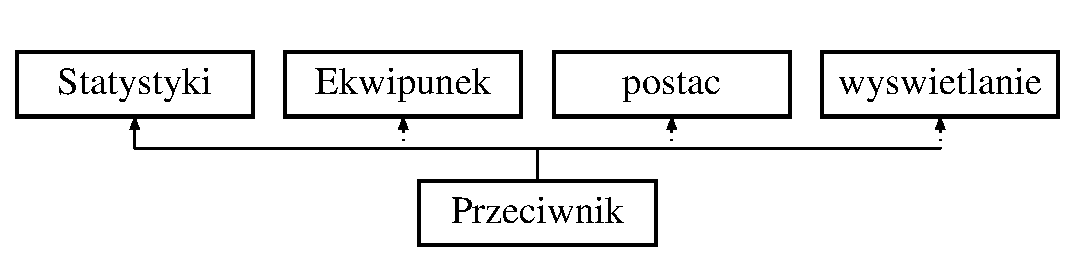
\includegraphics[height=2.000000cm]{class_przeciwnik}
\end{center}
\end{figure}
\subsection*{Metody publiczne}
\begin{DoxyCompactItemize}
\item 
{\bfseries Przeciwnik} (string nazwa=\char`\"{}Przeciwnik\char`\"{}, int poziom=5)\hypertarget{class_przeciwnik_a43091d28a1e7d139ebba933d94dbe59b}{}\label{class_przeciwnik_a43091d28a1e7d139ebba933d94dbe59b}

\item 
void {\bfseries wybierz\+Postac} ()\hypertarget{class_przeciwnik_a369acda4edc4173d1c58cd2aa55ec6cb}{}\label{class_przeciwnik_a369acda4edc4173d1c58cd2aa55ec6cb}

\item 
double {\bfseries algorytm\+Obliczenia\+Procentu} (int p)\hypertarget{class_przeciwnik_a64f579efdbd6bcabeaa88cb9cdcb1fe5}{}\label{class_przeciwnik_a64f579efdbd6bcabeaa88cb9cdcb1fe5}

\item 
double {\bfseries opoznienie\+Ataku} (double predkosc, int poziom, double procent)\hypertarget{class_przeciwnik_a01bd6be88bc9ef3752ffcc86a7d05e8d}{}\label{class_przeciwnik_a01bd6be88bc9ef3752ffcc86a7d05e8d}

\item 
void {\bfseries poczatkowe\+Staty} (int w, int p)\hypertarget{class_przeciwnik_ae81284629684beda35651b8622a9c9b0}{}\label{class_przeciwnik_ae81284629684beda35651b8622a9c9b0}

\item 
void {\bfseries wyswietl\+Staty\+Postaci} ()\hypertarget{class_przeciwnik_ab4b6ff29fd093dee4e61077865a2c8c7}{}\label{class_przeciwnik_ab4b6ff29fd093dee4e61077865a2c8c7}

\item 
void {\bfseries ekwipunek\+Postaci} (string \hyperlink{classpostac}{postac})\hypertarget{class_przeciwnik_a7ee1e71b9fd1b1101f6f3b0784ea74eb}{}\label{class_przeciwnik_a7ee1e71b9fd1b1101f6f3b0784ea74eb}

\item 
void {\bfseries wyswietl\+Ekwipunek} ()\hypertarget{class_przeciwnik_a2d14a358e48602b37c98af43b3c71c8f}{}\label{class_przeciwnik_a2d14a358e48602b37c98af43b3c71c8f}

\end{DoxyCompactItemize}
\subsection*{Atrybuty publiczne}
\begin{DoxyCompactItemize}
\item 
string {\bfseries typ}\hypertarget{class_przeciwnik_a40151e7196a294d2a417dd1da5bb7390}{}\label{class_przeciwnik_a40151e7196a294d2a417dd1da5bb7390}

\item 
string {\bfseries nazwapostaci}\hypertarget{class_przeciwnik_a5890b728264911f16538cc321242de92}{}\label{class_przeciwnik_a5890b728264911f16538cc321242de92}

\item 
int {\bfseries poziompostaci}\hypertarget{class_przeciwnik_a1c475fc41c7f49cb7e59da7b3a500a07}{}\label{class_przeciwnik_a1c475fc41c7f49cb7e59da7b3a500a07}

\end{DoxyCompactItemize}


Dokumentacja dla tej klasy została wygenerowana z plików\+:\begin{DoxyCompactItemize}
\item 
Uzytkownik.\+h\item 
Przeciwnik.\+cpp\end{DoxyCompactItemize}

\hypertarget{class_statystyki}{}\section{Dokumentacja klasy Statystyki}
\label{class_statystyki}\index{Statystyki@{Statystyki}}
Diagram dziedziczenia dla Statystyki\begin{figure}[H]
\begin{center}
\leavevmode
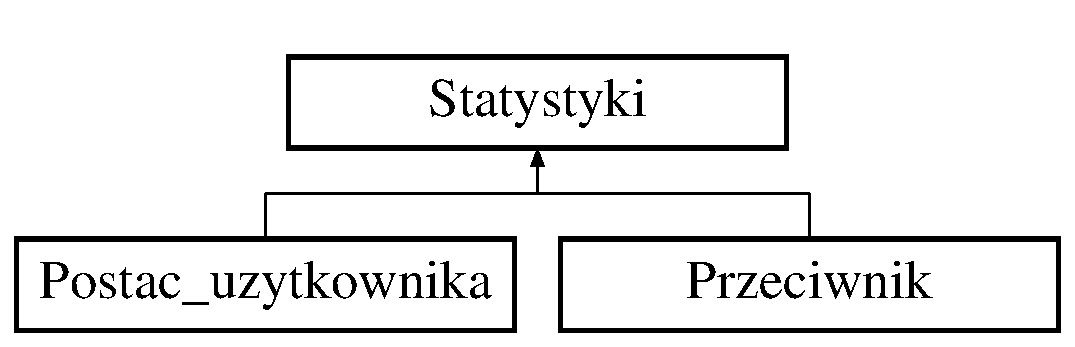
\includegraphics[height=2.000000cm]{class_statystyki}
\end{center}
\end{figure}
\subsection*{Atrybuty publiczne}
\begin{DoxyCompactItemize}
\item 
double {\bfseries obrazeniaataku}\hypertarget{class_statystyki_a3a4da2cc1e45164c741ab47b1beea1d2}{}\label{class_statystyki_a3a4da2cc1e45164c741ab47b1beea1d2}

\item 
double {\bfseries predkoscataku}\hypertarget{class_statystyki_a6dd1e90c5341b56d3c14be3e5b9a42fc}{}\label{class_statystyki_a6dd1e90c5341b56d3c14be3e5b9a42fc}

\item 
double {\bfseries odpornoscnamagie}\hypertarget{class_statystyki_a4a80a90f2604c8515891023194b219c3}{}\label{class_statystyki_a4a80a90f2604c8515891023194b219c3}

\item 
double {\bfseries pancerz}\hypertarget{class_statystyki_aee99c9a49f7e9439bcbd1b4ba929c787}{}\label{class_statystyki_aee99c9a49f7e9439bcbd1b4ba929c787}

\item 
double {\bfseries regeneracjazdrowia}\hypertarget{class_statystyki_a923d6e2bcd54e60a2503fc6363262aaf}{}\label{class_statystyki_a923d6e2bcd54e60a2503fc6363262aaf}

\item 
double {\bfseries zdrowie}\hypertarget{class_statystyki_a943bcebae41ee3f28aa9273a8d277bfc}{}\label{class_statystyki_a943bcebae41ee3f28aa9273a8d277bfc}

\item 
double {\bfseries mana}\hypertarget{class_statystyki_aed7bfef1a0d608a4634e2a241c92e8f5}{}\label{class_statystyki_aed7bfef1a0d608a4634e2a241c92e8f5}

\item 
double {\bfseries regeneracjamany}\hypertarget{class_statystyki_adf285bc31a4e56f42c03eb2a618b5888}{}\label{class_statystyki_adf285bc31a4e56f42c03eb2a618b5888}

\item 
double {\bfseries predkoscruchu}\hypertarget{class_statystyki_a93d335a339f20b3cabfd082aa09e38da}{}\label{class_statystyki_a93d335a339f20b3cabfd082aa09e38da}

\item 
double {\bfseries zzdrowie}\hypertarget{class_statystyki_a98bb51470e07606886a89f2289dfd115}{}\label{class_statystyki_a98bb51470e07606886a89f2289dfd115}

\item 
double {\bfseries rzdrowie}\hypertarget{class_statystyki_a6e1e421fe7d64305b193d64a4df8dc10}{}\label{class_statystyki_a6e1e421fe7d64305b193d64a4df8dc10}

\item 
double {\bfseries zmana}\hypertarget{class_statystyki_a072c834ff178954087efad2a9fc1e515}{}\label{class_statystyki_a072c834ff178954087efad2a9fc1e515}

\item 
double {\bfseries rmana}\hypertarget{class_statystyki_a6dcc8fefe27b66fdb9a4ec9ce0e9ec75}{}\label{class_statystyki_a6dcc8fefe27b66fdb9a4ec9ce0e9ec75}

\item 
double {\bfseries zatak}\hypertarget{class_statystyki_addde4e69058010e41430c6e64adbf492}{}\label{class_statystyki_addde4e69058010e41430c6e64adbf492}

\item 
double {\bfseries zpancerz}\hypertarget{class_statystyki_ad394e2cf0f6e62741c6a3801a6f790be}{}\label{class_statystyki_ad394e2cf0f6e62741c6a3801a6f790be}

\item 
double {\bfseries znamagie}\hypertarget{class_statystyki_abb2d2fc24214ec2f45dcd6cc5552bfbb}{}\label{class_statystyki_abb2d2fc24214ec2f45dcd6cc5552bfbb}

\end{DoxyCompactItemize}


Dokumentacja dla tej klasy została wygenerowana z pliku\+:\begin{DoxyCompactItemize}
\item 
Statystyki.\+h\end{DoxyCompactItemize}

\hypertarget{classwyswietlanie}{}\section{Dokumentacja klasy wyswietlanie}
\label{classwyswietlanie}\index{wyswietlanie@{wyswietlanie}}
Diagram dziedziczenia dla wyswietlanie\begin{figure}[H]
\begin{center}
\leavevmode
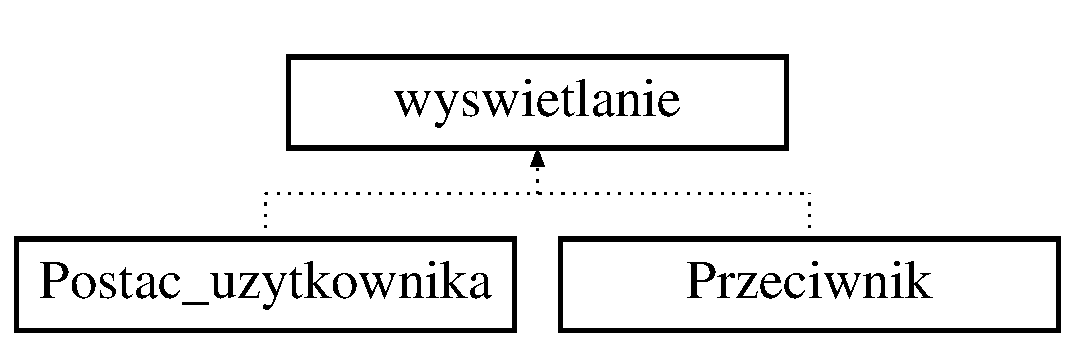
\includegraphics[height=2.000000cm]{classwyswietlanie}
\end{center}
\end{figure}
\subsection*{Metody publiczne}
\begin{DoxyCompactItemize}
\item 
virtual void {\bfseries wyswietl\+Staty\+Postaci} ()=0\hypertarget{classwyswietlanie_ab3d2fe917f699cfe71f91b595db5513c}{}\label{classwyswietlanie_ab3d2fe917f699cfe71f91b595db5513c}

\item 
virtual void {\bfseries wyswietl\+Ekwipunek} ()=0\hypertarget{classwyswietlanie_ae66e8ba8c3f792d7b6251f7eb7b17da5}{}\label{classwyswietlanie_ae66e8ba8c3f792d7b6251f7eb7b17da5}

\end{DoxyCompactItemize}


Dokumentacja dla tej klasy została wygenerowana z pliku\+:\begin{DoxyCompactItemize}
\item 
Wyswietlanie.\+h\end{DoxyCompactItemize}

%--- End generated contents ---

% Index
\backmatter
\newpage
\phantomsection
\clearemptydoublepage
\addcontentsline{toc}{chapter}{Indeks}
\printindex

\end{document}
